\documentclass[11pt,a4paper]{article}

% ── Packages ──────────────────────────────────────────────────────────
\usepackage[utf8]{inputenc}
\usepackage[T1]{fontenc}
\usepackage{lmodern}
\usepackage[margin=1in]{geometry}
\usepackage{amsmath,amssymb}
\usepackage{graphicx}
\usepackage{booktabs}
\usepackage{hyperref}
\usepackage{xcolor}
\usepackage{tikz}
\usetikzlibrary{arrows.meta,positioning,shapes.geometric,fit,calc}
\usepackage{caption}
\usepackage{subcaption}
\usepackage{enumitem}
\usepackage{multirow}
\usepackage{array}
\usepackage{tabularx}
\usepackage{float}
\usepackage{natbib}
\usepackage{authblk}
\usepackage{microtype}

\hypersetup{
    colorlinks=true,
    linkcolor=blue!60!black,
    citecolor=blue!60!black,
    urlcolor=blue!60!black,
}

% ── Inline tag command ────────────────────────────────────────────────
\newcommand{\etag}[1]{\texttt{[#1]}}

% ── Title ─────────────────────────────────────────────────────────────
\title{\textbf{Evoxtral: Expressive Tagged Transcription\\via Supervised Fine-Tuning and Rejection Sampling}}
\author[1]{Yongkang Zou}
\affil[1]{Mistral AI Online Hackathon 2026 --- W\&B Fine-Tuning Track}
\date{}

\begin{document}
\maketitle

% ══════════════════════════════════════════════════════════════════════
\begin{abstract}
Standard automatic speech recognition (ASR) systems discard paralinguistic and expressive information present in spoken audio, producing plain text that fails to capture sighs, laughs, hesitations, emotional tone, and other prosodic cues. We present \textbf{Evoxtral}, a LoRA adapter for \texttt{Voxtral-Mini-3B-2507}~\cite{voxtral} that produces transcriptions enriched with inline expressive audio tags drawn from the ElevenLabs v3 tag vocabulary~\cite{elevenlabs}. We apply a two-stage post-training pipeline: supervised fine-tuning (SFT) followed by rejection sampling fine-tuning (RAFT)~\cite{yuan2023rft}. SFT reduces word error rate (WER) by 33\% relative (6.64\%~$\to$~4.47\%) and increases Tag~F1 from 22.0\% to 67.2\%. The subsequent RAFT stage further improves Tag~F1 to 69.4\% and Tag~Recall to 72.7\% at a marginal WER cost. We release two model variants, a serverless inference API, and a live interactive demo.
\end{abstract}

% ══════════════════════════════════════════════════════════════════════
\section{Introduction}

Modern ASR pipelines excel at converting speech to text with low word error rates, yet they systematically strip out the expressive dimension of human communication. When a speaker sighs before a sentence, laughs nervously mid-phrase, or whispers for emphasis, these paralinguistic signals carry meaning that plain transcription cannot represent. This information is especially critical for downstream text-to-speech (TTS) synthesis: next-generation TTS systems such as ElevenLabs v3~\cite{elevenlabs} consume inline expressive tags to control prosody, affect, and delivery at a fine-grained level.

We ask: \emph{can a multimodal audio-language model be trained to produce ASR output that preserves expressive content through inline tags?} We answer affirmatively with \textbf{Evoxtral}, built on Voxtral-Mini-3B-2507~\cite{voxtral}.

\paragraph{Why Voxtral.} We chose Voxtral-Mini-3B as our base model for several reasons. First, as a \emph{generative} audio-language model (rather than a CTC or encoder-only ASR), Voxtral decodes transcriptions autoregressively---meaning it can naturally produce arbitrary inline tokens such as \etag{laughs} or \etag{nervous} within the text stream, without requiring architectural changes. Traditional ASR models constrain their output vocabulary to words and punctuation; Voxtral's LLM decoder has no such limitation. Second, Voxtral's compact 3B-parameter architecture makes LoRA fine-tuning feasible on a single A10G GPU within hackathon time constraints, while still delivering competitive ASR quality. Third, Voxtral was itself trained with post-training alignment (SFT~+~DPO~+~Online~DPO)~\cite{voxtral}, meaning the model is already instruction-following and amenable to further fine-tuning---a strong foundation for adding new capabilities. Finally, as a Mistral AI model released under Apache~2.0, Voxtral aligns with the hackathon's focus on the Mistral ecosystem and enables open redistribution of our adapters.

Our approach fine-tunes Voxtral-Mini-3B-2507 using parameter-efficient LoRA adapters~\cite{hu2021lora} on a synthetically generated dataset of expressive speech paired with tagged transcriptions.

\medskip
To illustrate the contrast, consider the following example:

\begin{quote}
\textbf{Standard ASR:} ``So I was thinking maybe we could try that new restaurant downtown. I mean if you're free this weekend.''

\textbf{Evoxtral:} ``\etag{nervous} So\ldots\ \etag{stammers} I was thinking maybe we could\ldots\ \etag{clears throat} try that new restaurant downtown? \etag{laughs nervously} I mean, if you're free this weekend?''
\end{quote}

\noindent The Evoxtral output captures hesitation, nervous laughter, and a throat clear---paralinguistic content that is acoustically present but conventionally discarded. We make the following contributions:

\begin{enumerate}[leftmargin=*,itemsep=2pt]
    \item A synthetic dataset of 1,010 expressive speech samples paired with tagged transcriptions across 17 ElevenLabs v3 tag types.
    \item A two-stage fine-tuning recipe (SFT~$\to$~RAFT) for expressive ASR using LoRA on Voxtral-Mini-3B.
    \item A custom evaluation benchmark, \textbf{Evoxtral-Bench}, with seven metrics covering both transcription accuracy and tag generation quality.
    \item Two released model variants optimized for different use cases: accuracy-critical (SFT) and expressiveness-critical (RL).
\end{enumerate}

% ══════════════════════════════════════════════════════════════════════
\section{Related Work}

\paragraph{Voxtral~\cite{voxtral}.} Voxtral-Mini-3B-2507 is a multimodal audio-language model released by Mistral~AI. It is built on a Whisper-based audio encoder fused with a Mistral language model backbone, trained via SFT, DPO, and online DPO. Our work builds directly on this foundation, adding expressive tagging capability via LoRA adaptation.

\paragraph{Reinforcement Learning for LLM-based ASR~\cite{grpo_asr}.} Shi et al.\ apply group relative policy optimization (GRPO) to LLM-based ASR, achieving an 18\% relative WER reduction without paired preference data. Closely related work~\cite{grpo_speech,rl_asr_tts,rl_audio_qa} further demonstrates that RL-based training consistently outperforms SFT alone for speech understanding tasks. Our RAFT stage is philosophically aligned with this line of work but uses rule-based rejection sampling rather than policy gradient methods, making it simpler to implement and more stable to train.

\paragraph{LoRA~\cite{hu2021lora}.} Low-rank adaptation inserts trainable low-rank matrices into the attention projections and feed-forward layers of a frozen base model, reducing the number of trainable parameters by orders of magnitude while matching full fine-tuning performance. We use LoRA with rank~64 and alpha~128, implemented via HuggingFace PEFT~\cite{peft}.

\paragraph{Rejection Sampling Fine-Tuning~\cite{yuan2023rft}.} Yuan et al.\ propose generating multiple model completions for each training input, scoring them with a reward function, and performing SFT on the highest-scoring completions. This approach is computationally simpler than policy gradient methods while still providing a reinforcement learning signal.

\paragraph{NEFTune~\cite{neftune}.} Jain et al.\ demonstrate that adding uniform random noise to embedding vectors during training improves instruction-following performance. We apply NEFTune with noise alpha~$=5.0$ during SFT to regularize training on our small dataset.

\paragraph{ElevenLabs v3 Audio Tags~\cite{elevenlabs}.} ElevenLabs v3 TTS introduces a structured vocabulary of inline expressive tags that control how synthesized speech is delivered. These tags---such as \etag{sighs}, \etag{laughs}, \etag{whispers}, and \etag{nervous}---are the target output vocabulary for Evoxtral.

\paragraph{ASR Evaluation~\cite{jiwer,morris2004wer}.} We compute WER and CER using the \texttt{jiwer} library~\cite{jiwer}, following standard definitions from Morris et al.~\cite{morris2004wer}.

% ══════════════════════════════════════════════════════════════════════
\section{Method}

\subsection{Dataset}

We construct a synthetic dataset of 1,010 audio samples generated using the ElevenLabs TTS v3 API~\cite{elevenlabs}. Each sample consists of a short spoken utterance (5--30\,s) paired with a reference tagged transcription containing inline expressive tags. The dataset covers 17~tag types: \etag{sighs}, \etag{laughs}, \etag{whispers}, \etag{nervous}, \etag{frustrated}, \etag{clears~throat}, \etag{pause}, \etag{excited}, \etag{stammers}, \etag{gasps}, \etag{sad}, \etag{angry}, \etag{calm}, \etag{crying}, \etag{shouts}, \etag{confused}, and \etag{scared}.

The dataset is split into 808~training, 101~validation, and 101~test samples. Tag frequency follows a long-tail distribution: \etag{pause} is the most common while \etag{confused} and \etag{scared} appear rarely. The Whisper-based audio encoder is kept frozen throughout training; only the language model backbone and multi-modal projector are fine-tuned.

\subsection{Stage 1: Supervised Fine-Tuning (SFT)}

We fine-tune Voxtral-Mini-3B-2507~\cite{voxtral} using LoRA~\cite{hu2021lora} with the configuration shown in Table~\ref{tab:sft_config}.

\begin{table}[h]
\centering
\caption{SFT hyperparameters.}
\label{tab:sft_config}
\begin{tabular}{@{}ll@{}}
\toprule
\textbf{Hyperparameter} & \textbf{Value} \\
\midrule
LoRA rank & 64 \\
LoRA alpha & 128 \\
LoRA dropout & 0.05 \\
Target modules & \texttt{q/k/v/o\_proj}, \texttt{gate/up/down\_proj}, \texttt{mm\_projector} \\
Learning rate & $2 \times 10^{-4}$ \\
LR schedule & Cosine decay \\
Epochs & 3 \\
Batch size & 2 (effective 16 via gradient accumulation $\times 8$) \\
NEFTune noise alpha & 5.0 \\
Precision & bf16 \\
Hardware & NVIDIA A10G (24\,GB) \\
Training time & $\sim$25 minutes \\
Trainable parameters & 124.8\,M / 4.8\,B (2.6\%) \\
\bottomrule
\end{tabular}
\end{table}

The SFT objective is standard next-token prediction (cross-entropy) on the tagged transcription tokens, conditioned on the audio encoder outputs. NEFTune~\cite{neftune} noise is applied to the input embeddings to reduce overfitting on the small training set.

\subsection{Stage 2: Rejection Sampling Fine-Tuning (RAFT)}

Following Yuan et al.~\cite{yuan2023rft} and inspired by Voxtral's own SFT$\to$DPO recipe~\cite{voxtral} and GRPO-based ASR work~\cite{grpo_asr}, we apply a rejection sampling stage to refine tag generation quality. The pipeline is illustrated in Figure~\ref{fig:raft_pipeline}.

\begin{figure}[t]
\centering
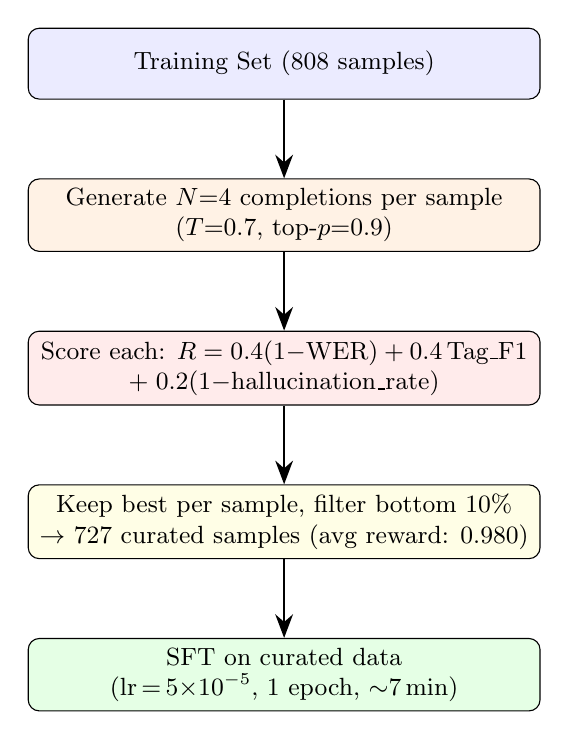
\begin{tikzpicture}[
    node distance=1.0cm,
    box/.style={draw, rounded corners, minimum width=6.5cm, minimum height=0.9cm, align=center, font=\small},
    arrow/.style={-{Stealth[length=3mm]}, thick},
]
    \node[box, fill=blue!8] (data) {Training Set (808 samples)};
    \node[box, fill=orange!10, below=of data] (gen) {Generate $N{=}4$ completions per sample\\($T{=}0.7$, top-$p{=}0.9$)};
    \node[box, fill=red!8, below=of gen] (score) {Score each: $R = 0.4(1{-}\text{WER}) + 0.4\,\text{Tag\_F1}$\\$+ \; 0.2(1{-}\text{hallucination\_rate})$};
    \node[box, fill=yellow!10, below=of score] (filter) {Keep best per sample, filter bottom 10\%\\$\to$ 727 curated samples (avg reward: 0.980)};
    \node[box, fill=green!10, below=of filter] (sft) {SFT on curated data\\(lr$\,{=}\,5{\times}10^{-5}$, 1 epoch, $\sim$7\,min)};

    \draw[arrow] (data) -- (gen);
    \draw[arrow] (gen) -- (score);
    \draw[arrow] (score) -- (filter);
    \draw[arrow] (filter) -- (sft);
\end{tikzpicture}
\caption{RAFT training pipeline. For each training sample, four completions are generated and scored by a rule-based reward function balancing transcription accuracy, tag quality, and hallucination avoidance. Only high-reward completions are retained for the final SFT pass.}
\label{fig:raft_pipeline}
\end{figure}

The reward function balances three objectives: transcription accuracy (WER), tag generation quality (Tag~F1), and avoidance of hallucinated tags:
\begin{equation}
    R = 0.4 \times (1 - \text{WER}) + 0.4 \times \text{Tag\_F1} + 0.2 \times (1 - \text{Hallucination\_Rate})
    \label{eq:reward}
\end{equation}

The 0.4/0.4/0.2 weighting reflects an equal priority on accuracy and expressiveness, with a penalty for hallucination. After filtering the bottom 10\% by reward (threshold: $R > 0.954$), 727 of the original 808 training samples remain with a mean reward of 0.980. The RAFT SFT stage trains for one epoch at a reduced learning rate of $5 \times 10^{-5}$, completing in approximately 7~minutes with a final training loss of 0.021.

The full two-stage pipeline overview is shown in Figure~\ref{fig:overview}.

\begin{figure}[t]
\centering
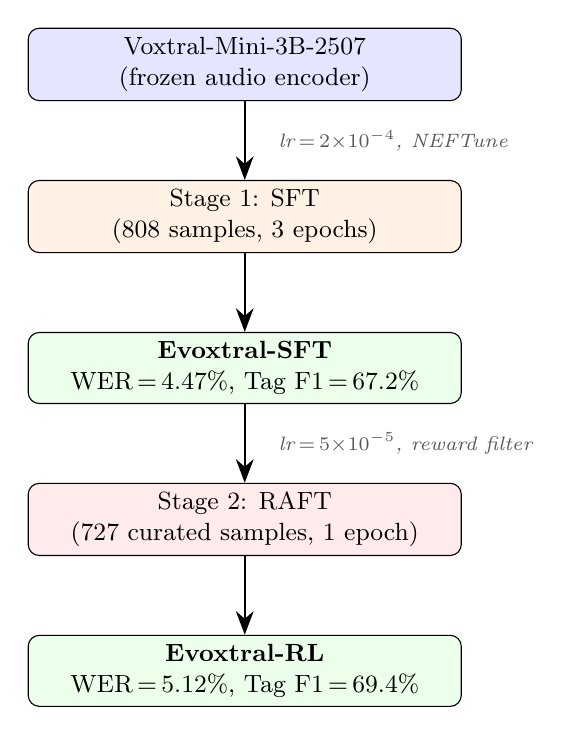
\begin{tikzpicture}[
    node distance=1.0cm,
    box/.style={draw, rounded corners, minimum width=5.5cm, minimum height=0.8cm, align=center, font=\small},
    result/.style={draw, rounded corners, minimum width=5.5cm, minimum height=0.8cm, align=center, font=\small, fill=green!8},
    arrow/.style={-{Stealth[length=3mm]}, thick},
    label/.style={font=\scriptsize\itshape, text=gray!70!black},
]
    \node[box, fill=blue!10] (base) {Voxtral-Mini-3B-2507\\(frozen audio encoder)};
    \node[box, fill=orange!10, below=of base] (sft) {Stage 1: SFT\\(808 samples, 3 epochs)};
    \node[result, below=of sft] (sft_r) {\textbf{Evoxtral-SFT}\\WER\,=\,4.47\%, Tag F1\,=\,67.2\%};
    \node[box, fill=red!8, below=of sft_r] (raft) {Stage 2: RAFT\\(727 curated samples, 1 epoch)};
    \node[result, below=of raft] (rl_r) {\textbf{Evoxtral-RL}\\WER\,=\,5.12\%, Tag F1\,=\,69.4\%};

    \draw[arrow] (base) -- (sft) node[midway, right=0.3cm, label] {lr\,$=$\,$2{\times}10^{-4}$, NEFTune};
    \draw[arrow] (sft) -- (sft_r);
    \draw[arrow] (sft_r) -- (raft) node[midway, right=0.3cm, label] {lr\,$=$\,$5{\times}10^{-5}$, reward filter};
    \draw[arrow] (raft) -- (rl_r);
\end{tikzpicture}
\caption{Full two-stage Evoxtral training pipeline from base Voxtral-Mini-3B to the two released model variants.}
\label{fig:overview}
\end{figure}

% ══════════════════════════════════════════════════════════════════════
\section{Evaluation}

\subsection{Evoxtral-Bench}

We evaluate on \textbf{Evoxtral-Bench}, a held-out benchmark of 50 test samples drawn from the 101-sample test split. We compute seven evaluation metrics:

\begin{itemize}[leftmargin=*,itemsep=1pt]
    \item \textbf{WER} (Word Error Rate, $\downarrow$) --- via \texttt{jiwer}~\cite{jiwer}, tags stripped before comparison
    \item \textbf{CER} (Character Error Rate, $\downarrow$) --- character-level accuracy via \texttt{jiwer}
    \item \textbf{Tag F1} ($\uparrow$) --- token-level F1 on predicted vs.\ reference tag multisets
    \item \textbf{Tag Precision} ($\uparrow$) --- fraction of predicted tags present in reference
    \item \textbf{Tag Recall} ($\uparrow$) --- fraction of reference tags captured by the model
    \item \textbf{Tag Hallucination Rate} ($\downarrow$) --- fraction of predicted tags absent from reference
    \item \textbf{Emphasis F1} ($\uparrow$) --- F1 on CAPITALIZED emphasis words
\end{itemize}

Per-tag F1 is additionally computed across all 17 tag types.

\subsection{Core Results}

\begin{table}[t]
\centering
\caption{Core evaluation results on Evoxtral-Bench (50 samples). Bold indicates best per metric. $\downarrow$ lower is better; $\uparrow$ higher is better.}
\label{tab:core_results}
\begin{tabular}{@{}lcccc@{}}
\toprule
\textbf{Metric} & \textbf{Base Voxtral} & \textbf{Evoxtral SFT} & \textbf{Evoxtral RL} & \textbf{Best} \\
\midrule
WER $\downarrow$ & 6.64\% & \textbf{4.47\%} & 5.12\% & SFT \\
CER $\downarrow$ & 2.72\% & \textbf{1.23\%} & 1.48\% & SFT \\
Tag F1 $\uparrow$ & 22.0\% & 67.2\% & \textbf{69.4\%} & RL \\
Tag Precision $\uparrow$ & 22.0\% & 67.4\% & \textbf{68.5\%} & RL \\
Tag Recall $\uparrow$ & 22.0\% & 69.4\% & \textbf{72.7\%} & RL \\
Emphasis F1 $\uparrow$ & 42.0\% & 84.0\% & \textbf{86.0\%} & RL \\
Tag Hallucination $\downarrow$ & 0.0\% & \textbf{19.3\%} & 20.2\% & SFT \\
\bottomrule
\end{tabular}
\end{table}

The base Voxtral model achieves 22.0\% Tag~F1, suggesting some limited native capability to produce expressive tokens but with low precision and recall. SFT provides the dominant improvement: WER decreases by 33\% relative (6.64\%~$\to$~4.47\%) and Tag~F1 increases by 45~percentage points (22.0\%~$\to$~67.2\%). RAFT further refines tag metrics: Tag~F1 improves by 2.2\,pp (67.2\%~$\to$~69.4\%), Tag~Recall by 3.3\,pp (69.4\%~$\to$~72.7\%), and Emphasis~F1 by 2.0\,pp (84.0\%~$\to$~86.0\%). However, RAFT introduces a small WER regression (4.47\%~$\to$~5.12\%), reflecting a Pareto tradeoff between transcription accuracy and expressive richness.

Tag hallucination---predicted tags absent from the reference---is 19.3\% for SFT and 20.2\% for RL. The base model has 0\% hallucination because it rarely predicts any tags at all.

\subsection{Per-Tag F1 Breakdown}

\begin{table}[t]
\centering
\caption{Per-tag F1 scores for SFT and RL on Evoxtral-Bench. Support indicates the number of test samples containing each tag.}
\label{tab:per_tag}
\begin{tabular}{@{}lcccc@{}}
\toprule
\textbf{Tag} & \textbf{SFT F1} & \textbf{RL F1} & \textbf{$\Delta$} & \textbf{Support} \\
\midrule
\etag{sighs} & 1.000 & 1.000 & --- & 9 \\
\etag{clears throat} & 0.889 & \textbf{1.000} & +12.5\% & 8 \\
\etag{gasps} & 0.957 & 0.957 & --- & 12 \\
\etag{pause} & 0.885 & \textbf{0.902} & +1.9\% & 25 \\
\etag{nervous} & 0.800 & \textbf{0.846} & +5.8\% & 13 \\
\etag{stammers} & \textbf{0.889} & 0.842 & $-$5.3\% & 8 \\
\etag{laughs} & 0.800 & \textbf{0.815} & +1.9\% & 12 \\
\etag{sad} & 0.667 & \textbf{0.750} & +12.4\% & 4 \\
\etag{whispers} & 0.636 & \textbf{0.667} & +4.9\% & 13 \\
\etag{crying} & \textbf{0.750} & 0.571 & $-$23.9\% & 5 \\
\etag{excited} & \textbf{0.615} & 0.571 & $-$7.2\% & 5 \\
\etag{shouts} & 0.400 & \textbf{0.500} & +25.0\% & 3 \\
\etag{calm} & 0.200 & \textbf{0.400} & +100\% & 6 \\
\etag{frustrated} & 0.444 & 0.444 & --- & 3 \\
\etag{angry} & 0.667 & 0.667 & --- & 2 \\
\etag{confused} & 0.000 & 0.000 & --- & 1 \\
\etag{scared} & 0.000 & 0.000 & --- & 1 \\
\bottomrule
\end{tabular}
\end{table}

RAFT improves 9~tags, maintains 4~stable, and regresses on~3 (Table~\ref{tab:per_tag}). The largest gains are observed for \etag{calm} (+100\%, 0.200~$\to$~0.400), \etag{shouts} (+25.0\%), \etag{clears~throat} (+12.5\%), and \etag{sad} (+12.4\%). Regressions are noted for \etag{crying} ($-$23.9\%), \etag{excited} ($-$7.2\%), and \etag{stammers} ($-$5.3\%). The two zero-F1 tags (\etag{confused}, \etag{scared}) each appear only once in the test set, making estimation unreliable.

% ══════════════════════════════════════════════════════════════════════
\section{Analysis and Discussion}

\paragraph{SFT as the primary driver of improvement.} The SFT stage accounts for the vast majority of the performance gain: WER drops 33\% relative and Tag~F1 increases by 45~percentage points. This aligns with findings from GRPO-based ASR work~\cite{grpo_asr,grpo_speech,rl_asr_tts} suggesting that a well-supervised initial adaptation is a strong foundation for subsequent RL refinement.

\paragraph{The WER--Tag tradeoff.} RAFT improves tag metrics at the cost of a modest WER regression (4.47\%~$\to$~5.12\%). This suggests the existence of a Pareto frontier between transcription accuracy and expressive richness: optimizing for tag generation pushes the model toward producing more tags, which can introduce minor word-level errors. This motivates releasing two model variants---Evoxtral-SFT for accuracy-critical applications (e.g., professional transcription) and Evoxtral-RL for expressiveness-critical applications (e.g., downstream TTS synthesis with ElevenLabs v3~\cite{elevenlabs}).

\paragraph{Tag hallucination.} Approximately 20\% of predicted tags are not present in the reference transcription. Hallucination may occur when the model infers an expressive tone from acoustic cues that are present in the audio but absent or differently annotated in the reference. This may partly reflect annotation noise in synthetic data rather than pure model error. Future work should address this with contrastive or calibration-based training objectives.

\paragraph{Effect of NEFTune.} Applying NEFTune~\cite{neftune} with noise alpha~$=5.0$ during SFT provided a regularization benefit on the small 808-sample training set, consistent with Jain et al.'s findings on instruction-following tasks. Ablating this component was not feasible within hackathon time constraints but remains a planned analysis.

\paragraph{Rare tag performance.} Tags with very low test support (\etag{confused}, \etag{scared}, support\,$=$\,1) have zero~F1, which is uninformative. Tags with support 2--6 show high variance in F1 estimates. A larger, more balanced evaluation set would provide more reliable per-tag metrics.

\paragraph{Reward function design.} The RAFT reward (Equation~\ref{eq:reward}) explicitly encodes the design preference for equal weight on accuracy and expressiveness. The 0.2 weight on hallucination acts as a weak regularizer. An ablation across reward weightings would quantify the sensitivity of the final model to this design choice.

% ══════════════════════════════════════════════════════════════════════
\section{Limitations}

\begin{itemize}[leftmargin=*,itemsep=2pt]
    \item \textbf{Synthetic training data.} All 1,010 samples are synthesized using ElevenLabs TTS v3~\cite{elevenlabs}. The acoustic properties of synthetic speech differ from natural human speech. Performance on natural speech recordings may differ.
    \item \textbf{Tag hallucination.} Approximately 20\% of predicted tags in the RL model are not present in the reference, which may limit applicability in settings requiring precise expressive annotation.
    \item \textbf{Rare tag coverage.} Seventeen tag types are represented, but several occur in fewer than 5 test samples. Per-tag F1 estimates for rare categories are unreliable.
    \item \textbf{English only.} The dataset and training are English-only. Generalization to other languages is not evaluated.
    \item \textbf{Small dataset.} 808 training samples is a small fine-tuning set. Scaling to thousands of examples with natural speech could substantially improve performance.
    \item \textbf{Evaluation scope.} Evoxtral-Bench covers 50 test samples. A larger evaluation set would yield more statistically robust estimates.
\end{itemize}

% ══════════════════════════════════════════════════════════════════════
\section{Conclusion}

We presented Evoxtral, a LoRA-adapted version of Voxtral-Mini-3B-2507~\cite{voxtral} that produces expressive tagged transcriptions using ElevenLabs v3 audio tags~\cite{elevenlabs}. Our two-stage training pipeline---SFT followed by RAFT~\cite{yuan2023rft}---demonstrates that expressive tagging capability can be effectively injected into a pre-trained ASR model with parameter-efficient fine-tuning~\cite{hu2021lora,peft}.

SFT achieves a 33\% relative WER reduction and a 45~percentage-point improvement in Tag~F1 over the base model. RAFT further improves tag recall and F1 by targeting tag generation quality directly through a rule-based reward signal, at a modest transcription accuracy cost. The two resulting model variants cover a Pareto frontier between accuracy and expressiveness, allowing practitioners to select the appropriate trade-off for their application.

Future directions include: (1)~collecting natural speech data with crowd-sourced expressive annotations to reduce the synthetic data gap; (2)~replacing RAFT with GRPO~\cite{grpo_asr} or DPO~\cite{voxtral} for more sample-efficient RL training; (3)~expanding to multilingual settings leveraging Voxtral's multilingual audio encoder; and (4)~developing joint ASR+TTS evaluation protocols that measure downstream TTS quality when Evoxtral output is used as input to ElevenLabs v3~\cite{elevenlabs}.

% ══════════════════════════════════════════════════════════════════════
\bibliographystyle{plainnat}

\begin{thebibliography}{12}

\bibitem[{Mistral AI}(2025)]{voxtral}
Mistral AI.
\newblock Voxtral.
\newblock \emph{arXiv preprint arXiv:2507.13264}, 2025.
\newblock \url{https://arxiv.org/abs/2507.13264}

\bibitem[{Shi et~al.}(2025)]{grpo_asr}
Shi, B. et~al.
\newblock Group relative policy optimization for speech recognition.
\newblock \emph{arXiv preprint arXiv:2509.01939}, 2025.
\newblock \url{https://arxiv.org/abs/2509.01939}

\bibitem[{Hu et~al.}(2022)]{hu2021lora}
Hu, E.J., Shen, Y., Wallis, P., Allen-Zhu, Z., Li, Y., Wang, S., Wang, L., and Chen, W.
\newblock {LoRA}: Low-rank adaptation of large language models.
\newblock In \emph{Proceedings of ICLR}, 2022.
\newblock \url{https://arxiv.org/abs/2106.09685}

\bibitem[{Yuan et~al.}(2023)]{yuan2023rft}
Yuan, Z., Yuan, H., Li, C., Dong, G., Tan, C., and Zhou, C.
\newblock Scaling relationship on learning mathematical reasoning with large language models.
\newblock \emph{arXiv preprint arXiv:2308.01825}, 2023.
\newblock \url{https://arxiv.org/abs/2308.01825}

\bibitem[{Jain et~al.}(2024)]{neftune}
Jain, N., Chiang, P., Yeh, Y., Kirchenbauer, J., et~al.
\newblock {NEFTune}: Noisy embeddings improve instruction finetuning.
\newblock In \emph{Proceedings of ICLR}, 2024.
\newblock \url{https://arxiv.org/abs/2310.05914}

\bibitem[{ElevenLabs}(2025)]{elevenlabs}
ElevenLabs.
\newblock Text-to-speech v3 audio tags.
\newblock ElevenLabs Developer Documentation, 2025.
\newblock \url{https://elevenlabs.io/docs/api-reference/text-to-speech}

\bibitem[{JiWER}(2024)]{jiwer}
JiWER: Evaluate your speech recognition system.
\newblock Python library for ASR evaluation metrics.
\newblock \url{https://github.com/jitsi/jiwer}

\bibitem[{}(2025a)]{grpo_speech}
Advancing speech understanding in speech-aware language models with {GRPO}.
\newblock \emph{arXiv preprint arXiv:2509.16990}, 2025.
\newblock \url{https://arxiv.org/abs/2509.16990}

\bibitem[{}(2025b)]{rl_asr_tts}
Explore the reinforcement learning for {LLM}-based {ASR} and {TTS} system.
\newblock \emph{arXiv preprint arXiv:2509.18569}, 2025.
\newblock \url{https://arxiv.org/abs/2509.18569}

\bibitem[{Mangrulkar et~al.}(2022)]{peft}
Mangrulkar, S., Gugger, S., Debut, L., Belkada, Y., Paul, S., and Bossan, B.
\newblock {PEFT}: State-of-the-art parameter-efficient fine-tuning methods.
\newblock HuggingFace, 2022.
\newblock \url{https://github.com/huggingface/peft}

\bibitem[{Morris et~al.}(2004)]{morris2004wer}
Morris, A.C., Maier, V., and Green, P.
\newblock From {WER} and {RIL} to {MER} and {WIL}: Improved evaluation measures for connected speech recognition.
\newblock In \emph{Proceedings of INTERSPEECH}, 2004.

\bibitem[{}(2025c)]{rl_audio_qa}
Reinforcement learning outperforms supervised fine-tuning: A case study on audio question answering.
\newblock \emph{arXiv preprint arXiv:2503.11197}, 2025.
\newblock \url{https://arxiv.org/abs/2503.11197}

\end{thebibliography}

\end{document}
